\clearpage
\section{الرئيسية ومسارك بحسب المسؤولية}
\label{sec:correspondence-feature-home}

تجمع الرئيسية مداخل العمل والمتابعة. يحدد العمل المسند إليك نقطة البداية؛ فقد تكون مُعِدّاً لكتاب، أو مراجعاً لمسودة، أو معتمداً، أو مستلماً، أو موظف ديوان. هذه مسؤوليات في سير العمل، وليست أسماء أدوار يجب إنشاؤها بهذه الصيغة.

\begin{rcnote}[مثال: شركة الأفق]
يتحقق عمر من صفته عند ① ثم يفتح الصندوق من ② لاستكمال مسودة طلب الزيارة. وتستخدم سارة «بانتظار اعتمادي» عند ③ إذا وصل إليها طلب اعتماد؛ فمنصبها وحده لا يجعلها معتمدة لكل كتاب.
\end{rcnote}
\begin{figure}[H]
\centering
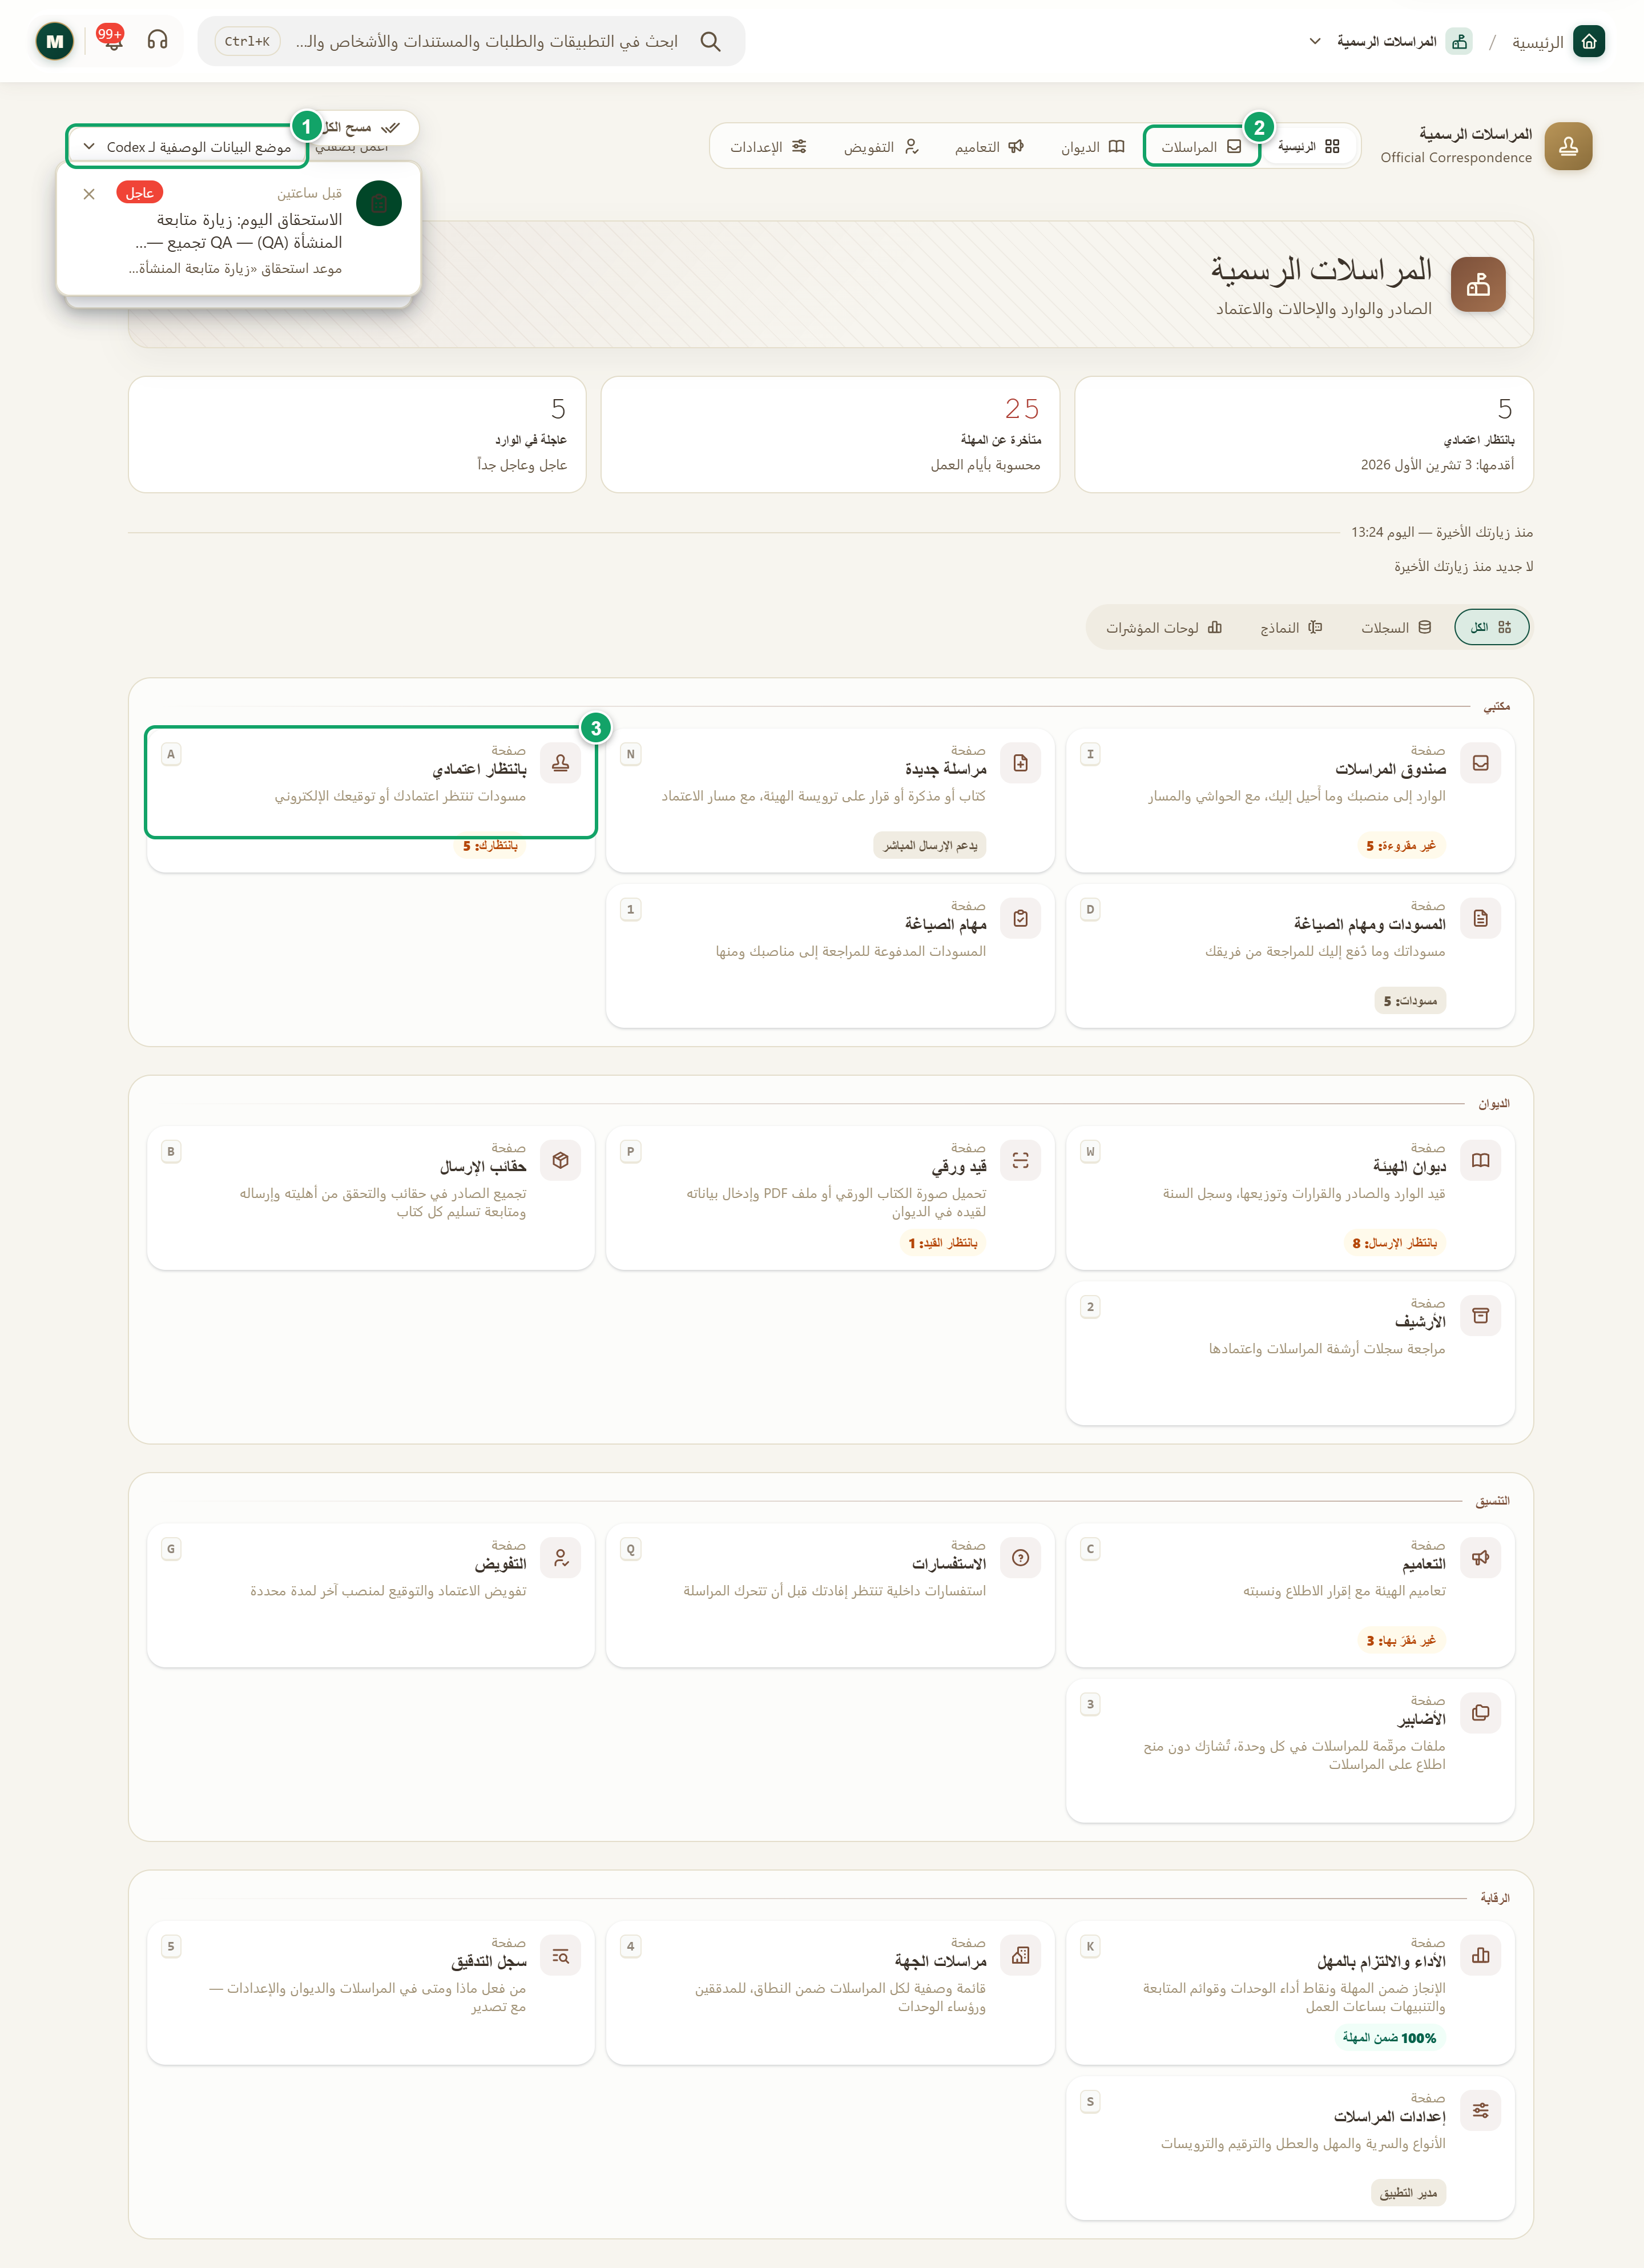
\includegraphics[width=0.95\linewidth,height=0.72\textheight,keepaspectratio]{figures/screens/ch07-home-ar.png}
\caption{الرئيسية ومداخل العمل}
\label{fig:correspondence-home-screen}
\shotnote{تجمع الرئيسية مداخل العمل بحسب المسؤولية، وتعرض أعداداً تساعد على بدء المتابعة. الأرقام تخص سجلات الاختبار ولا تصف مثال الأفق. ① «الصفة» لاختيار المنصب الذي تعمل باسمه. ② «المراسلات» لفتح الصندوق. ③ «بانتظار اعتمادي» لعرض طلبات الاعتماد المتاحة لك.}
\end{figure}


\begin{table}[H]
\centering
\caption{أين تبدأ بحسب عملك؟}
\label{tab:correspondence-responsibilities}
\begin{tabularx}{\linewidth}{R{4.2cm} Y}
\rcHeaderRow
\thh{المسؤولية} & \thh{نقطة البداية}\\
المُعِدّ & ابدأ من «مراسلة جديدة» للإعداد، ومن «المسودات ومهام الصياغة» لاستكمال عمل محفوظ.\\
مراجع الصياغة & افتح «مهام الصياغة» لتعرف المسودات التي دُفعت للمراجعة. المراجعة ليست اعتماداً نهائياً.\\
المعتمد & افتح «بانتظار اعتمادي» وافحص الطلب الموجّه إليك.\\
المستلم & افتح «صندوق المراسلات» ثم «الواردة»؛ أما «نسخ للعلم» فتساعدك على تمييز ما وصلك للاطلاع.\\
موظف الديوان & ابدأ من «ديوان الهيئة» عند توافر صلاحية القيد.\\
مسؤول التهيئة & افتح «إعدادات المراسلات» عند توافر صلاحية الإدارة.\\
\end{tabularx}
\end{table}

\begin{enumerate}
\item افتح تطبيق «المراسلات الرسمية» من مشغّل التطبيقات.
\item اقرأ «أعمل بصفتي»، ثم افتح مدخل العمل الذي يخص مسؤوليتك من الجدول.
\item تحقق من عنوان الصفحة والمجلد؛ فـ«بانتظار اعتمادي» و«المسودات ومهام الصياغة» مدخلان إلى عروض داخل الصندوق.
\end{enumerate}

\textbf{تحقق:} سمِّ مسؤوليتك ونقطة بدايتك قبل متابعة الدليل. إذا غاب الديوان أو الإعدادات، راجع الصلاحية مع المسؤول؛ ولا تستنتج من غياب المدخل أن التطبيق معطّل.

\clearpage
\section{الصفة والصلاحيات}
\label{sec:correspondence-feature-capacity}

الصفة هي المنصب الذي تتعامل مع المراسلات باسمه. قد يرتبط حسابك بأكثر من منصب، وقد يتاح لك منصب آخر بتفويض سارٍ. تغيير الصفة لا يمنحك صلاحية جديدة؛ وتبقى الإجراءات المتاحة مرتبطة بالمراسلة والتعيين والتفويض والصلاحيات.

\begin{rcnote}[مثال: شركة الأفق]
يختار عمر منصبه «منسق عمليات» عند ①، ثم يفتح «المسودات» عند ② ليتابع طلب الزيارة. وإذا فُوّض لاحقاً عن منصب آخر، يميّز العمل نيابةً عنه من عمل منصبه الأصلي.
\end{rcnote}
\begin{figure}[H]
\centering
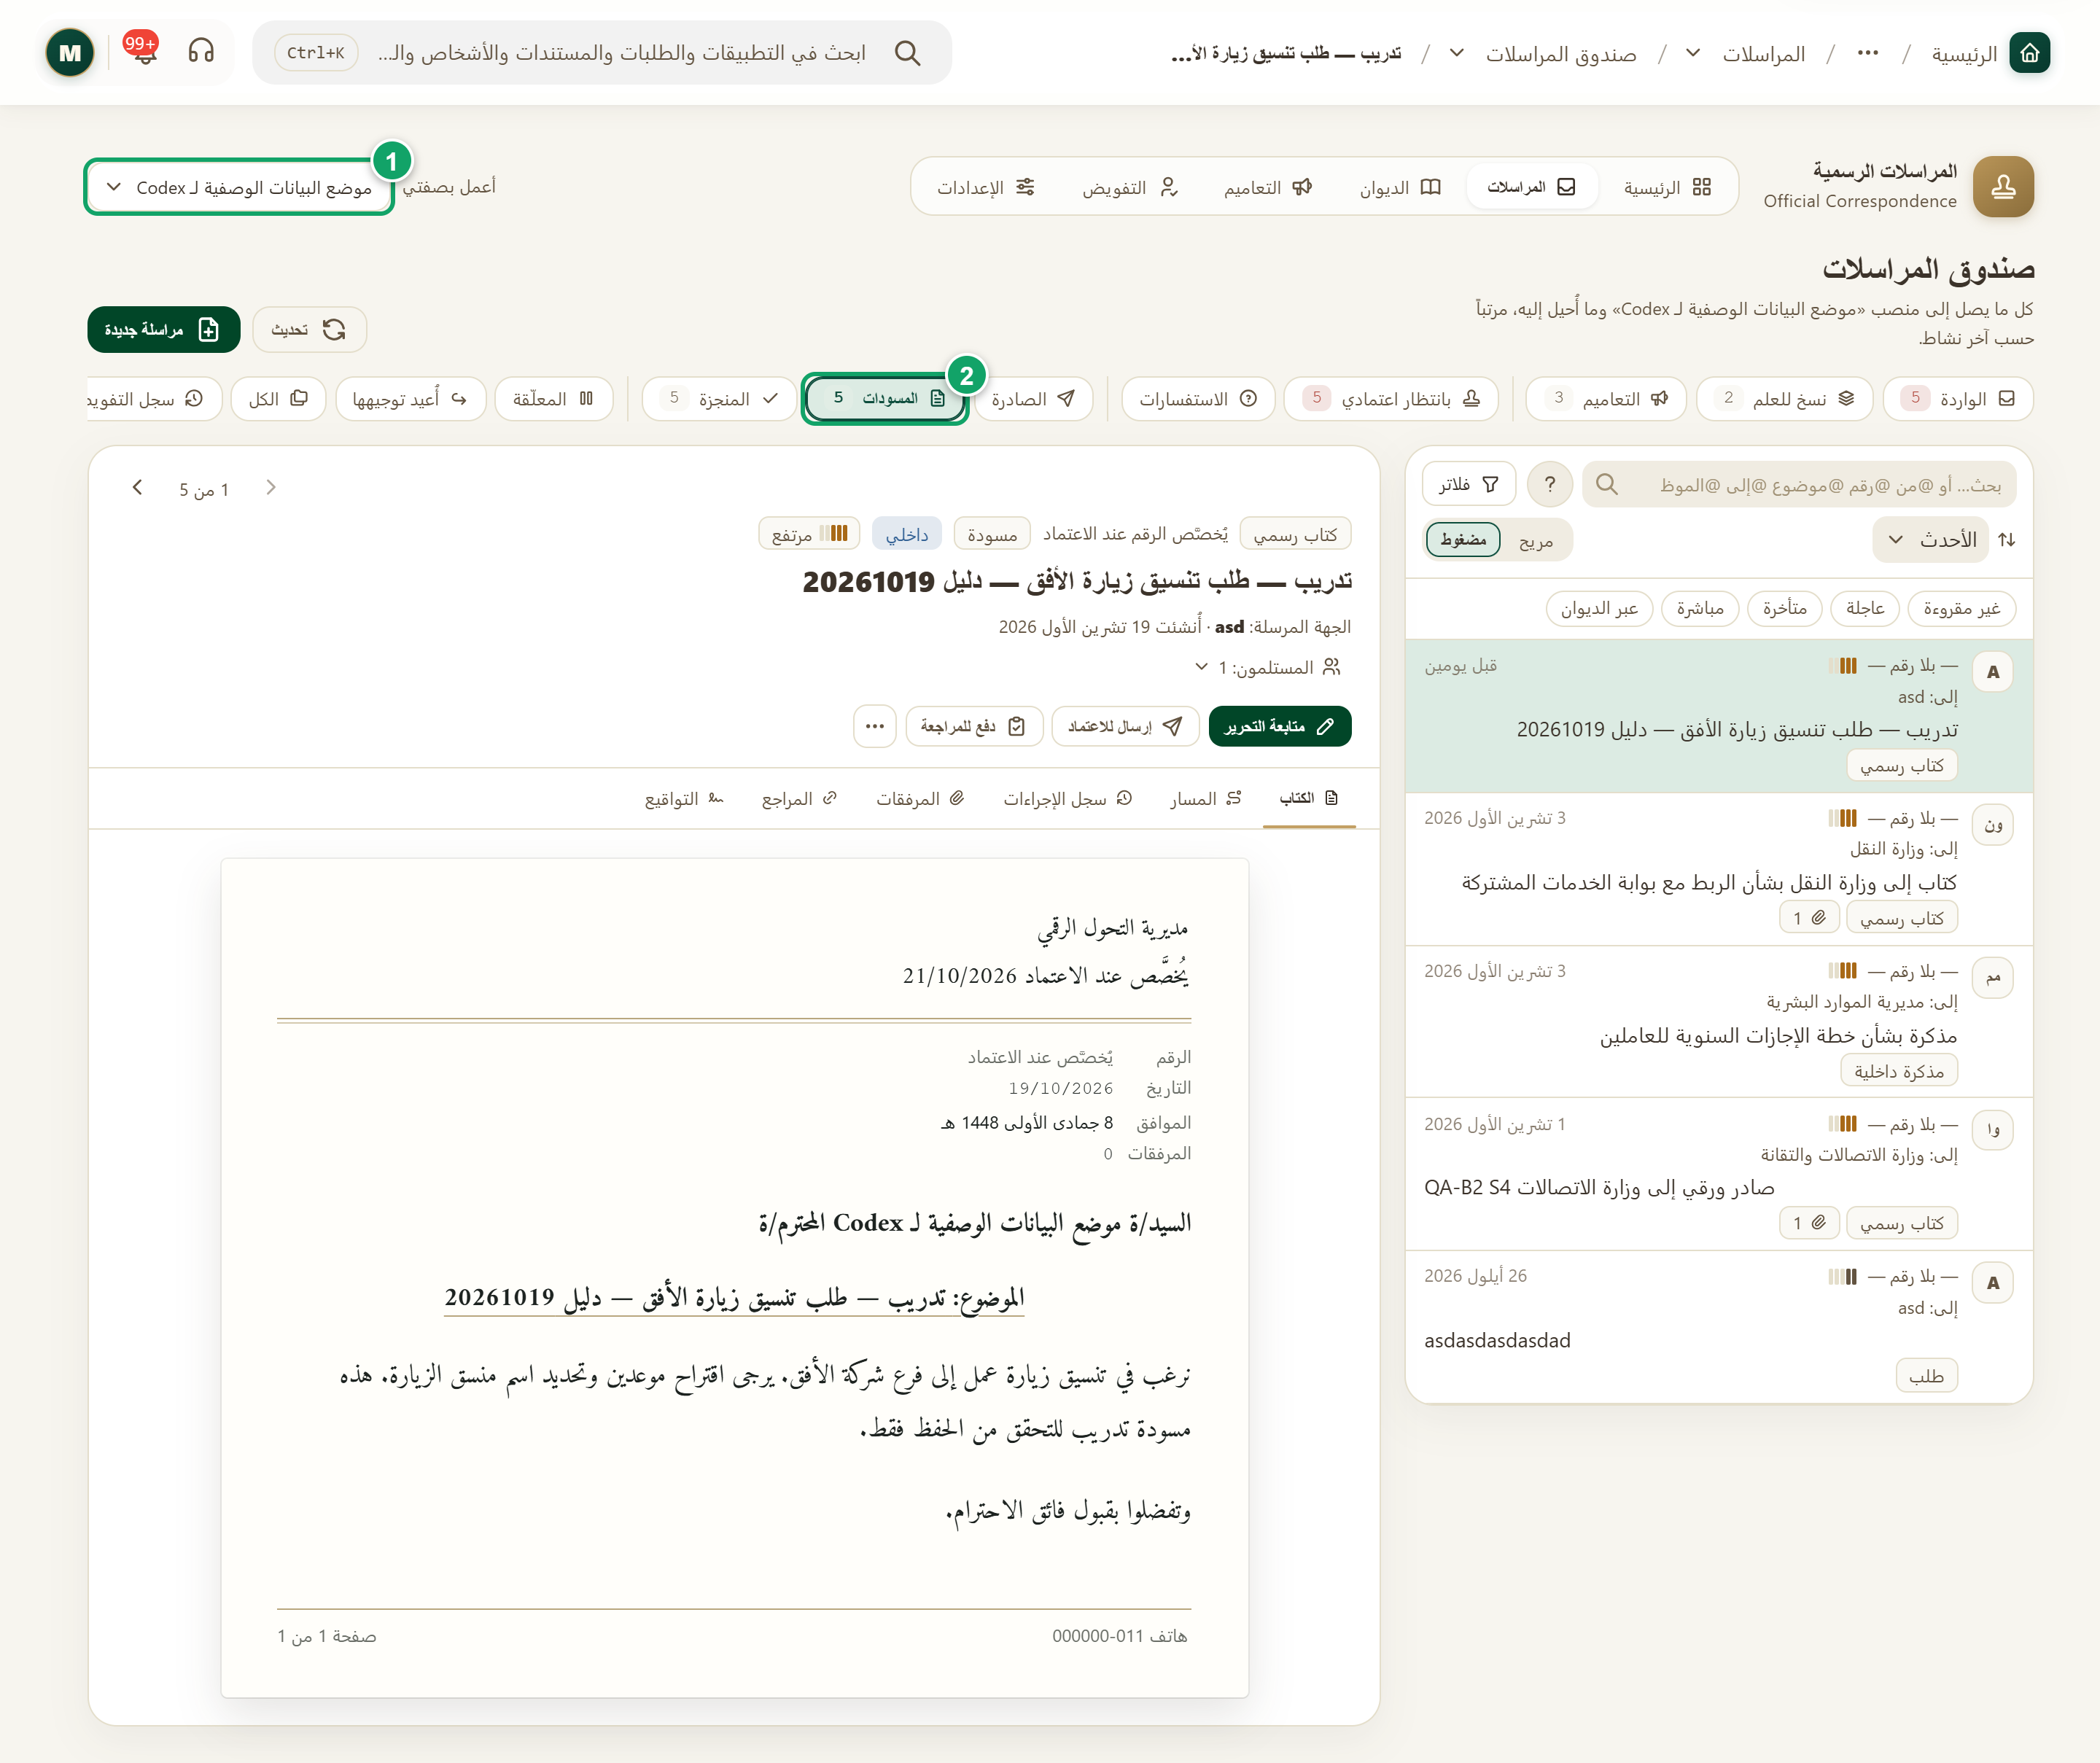
\includegraphics[width=0.95\linewidth,height=0.72\textheight,keepaspectratio]{figures/screens/ch07-capacity-ar.png}
\caption{الصفة ومجلد المسودات}
\label{fig:correspondence-capacity-screen}
\shotnote{تعرض الصورة المنصب المختار وسياق المجلد الذي تتابعه، مع مسودة اختبار مفتوحة. وجود مسودة في الصندوق لا يعني أنها أُرسلت للاعتماد. ① «الصفة» لتحديد المنصب قبل متابعة العمل. ② «المسودات» للعودة إلى الكتب التي ما زالت في الإعداد.}
\end{figure}


\begin{enumerate}
\item افتح «المراسلات الرسمية» وابحث عن «أعمل بصفتي».
\item إذا ظهرت قائمة مناصب، اختر المنصب المطلوب واقرأ اسمه بعد الاختيار. عند إتاحة منصب واحد يظهر الاسم دون قائمة تبديل.
\item عند العمل بالتفويض، افحص عبارة «نيابةً عن» وتاريخ انتهاء التفويض.
\item افتح «صندوق المراسلات» وتحقق من سياق المنصب قبل اختيار مراسلة.
\end{enumerate}

\textbf{تحقق ومعالجة المشكلة:} اذكر المنصب الذي تعمل باسمه، وهل تعمل بالتفويض. إذا غاب المنصب المطلوب، اطلب التحقق من تعيينك أو سريان التفويض وشروطه؛ لا تُنشئ مراسلة باسم منصب آخر لتجاوز المشكلة.

\clearpage
\section{صندوق المراسلات ودورة العمل}
\label{sec:correspondence-feature-tray}

يجمع «صندوق المراسلات» العمل المتاح لك في مجلدات. المجلد وسيلة للعثور على العمل، أما الحالة فتصف مرحلة المراسلة؛ لذلك لا تخلط «بانتظار اعتمادي» مع حالة جميع المراسلات، ولا تعتبر الصدور دليلاً على التسليم أو الإنجاز.

\begin{rcnote}[مثال: شركة الأفق]
تفتح سارة «الواردة» عند ① للعثور على مراسلة تخص زيارة فرع حلب، ثم تبحث عن موضوعها في ②. تستخدم «فلاتر» عند ③ إذا احتاجت إلى تضييق النتائج، وتعيد تحميل القائمة من ④ قبل فحص النتيجة.
\end{rcnote}
\begin{figure}[H]
\centering
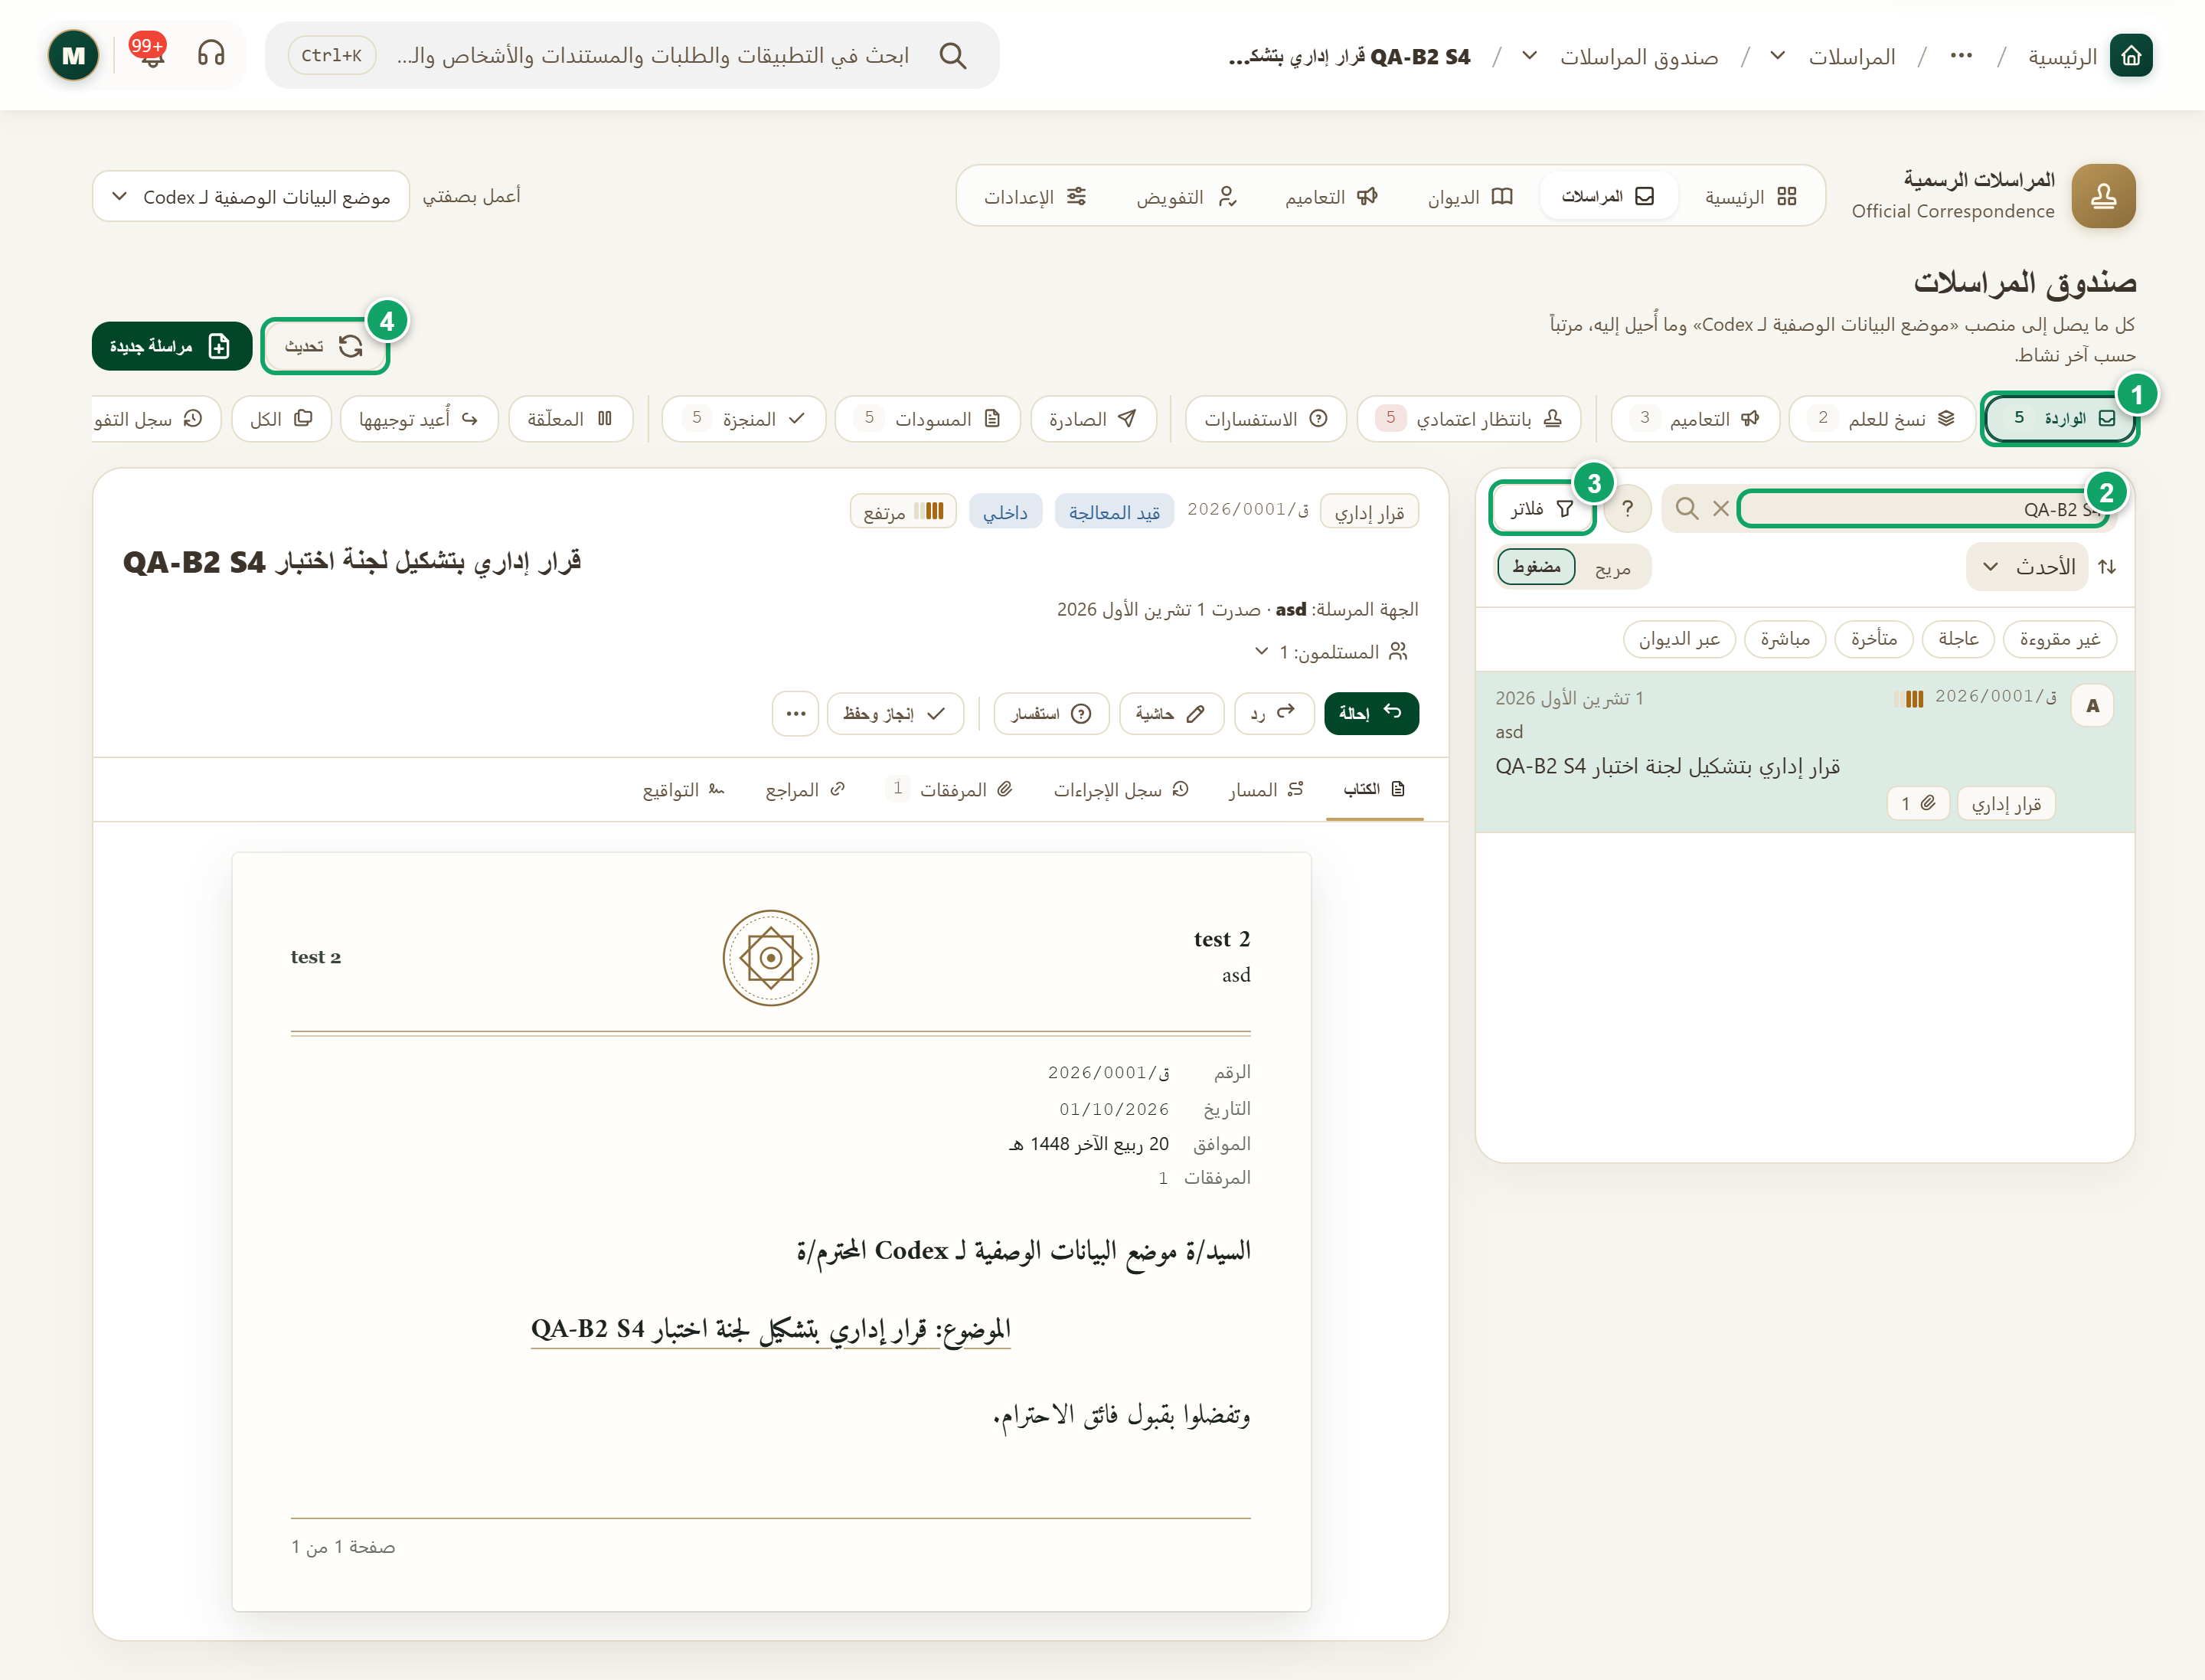
\includegraphics[width=0.95\linewidth,height=0.72\textheight,keepaspectratio]{figures/screens/ch07-tray-ar.png}
\caption{البحث في صندوق المراسلات}
\label{fig:correspondence-tray-screen}
\shotnote{تعرض الصورة نتيجة بحث محدد وكتاب اختبار مفتوحاً، فتستطيع مقارنة الحالة والأولوية والسرية دون الخلط بينها. البحث يضيّق القائمة، ولا يغيّر حالة الكتاب. ① «الواردة» لاختيار المجلد. ② خانة البحث للعثور على موضوع معلوم. ③ «فلاتر» لتضييق النتائج. ④ «تحديث» لإعادة تحميل القائمة.}
\end{figure}


\begin{table}[H]
\centering
\caption{كيف تقرأ بيانات المراسلة؟}
\label{tab:correspondence-reading}
\begin{tabularx}{\linewidth}{R{4.2cm} Y}
\rcHeaderRow
\thh{البيان} & \thh{ما الذي تفهمه منه؟}\\
نوع المراسلة & يحدد تصنيف الكتاب وفق الأنواع التي هيأتها المؤسسة؛ لا تفترض أن قائمة الأنواع موحدة في كل مؤسسة.\\
الحالة & تظهر تسميات مثل «مسودة»، و«بانتظار الاعتماد»، و«أُعيدت للتعديل»، و«صادرة»، و«قيد المعالجة»، و«منجزة»، و«مرفوضة»، و«ملغى». لا تمثل هذه القائمة مساراً إلزامياً واحداً.\\
الأولوية & تساعدك تسميات مثل «عاجل» و«عاجل جداً» على ترتيب المتابعة؛ ولا تعني منح صلاحية إضافية.\\
السرية & تميّز تصنيف الاطلاع، مثل «عام» و«داخلي» و«سري». لا تجعلها مرادفاً للأولوية.\\
المهلة & تساعدك على معرفة ما يستحق المتابعة؛ افحص تاريخ الاستحقاق وما إذا كانت المهلة موقوفة.\\
\end{tabularx}
\end{table}

\begin{enumerate}
\item افتح «صندوق المراسلات»، ثم اختر «الواردة» أو «المسودات» أو «بانتظار اعتمادي» بحسب عملك.
\item اكتب كلمة من موضوع كتاب معلوم في البحث، ثم افحص النتائج. يمكنك استخدام «فلاتر» أو أحد الفلاتر السريعة مثل «غير مقروءة» و«عاجلة».
\item امسح البحث وألغِ الفلتر إذا لم تظهر المراسلة، ثم تحقق من الصفة والمجلد. استخدم «تحديث» لإعادة تحميل القائمة.
\item افتح مراسلة متاحة واقرأ موضوعها وحالتها وأولويتها وسريتها قبل اتخاذ إجراء.
\end{enumerate}

\textbf{تمرين وتحقق:} انتقل من «الواردة» إلى «المسودات» ثم عد، وجرّب بحثاً ثم امسحه. تحقق من تغير المجلد وعودة القائمة؛ وإذا كانت فارغة، سجّل ذلك ولا تعتبره دليلاً على عدم وجود مراسلات في المؤسسة. عند ظهور «تعذّر تحميل المجلد»، استخدم «إعادة المحاولة»؛ فالخطأ ليس نتيجة بحث فارغة.
